\chapter{Fundamentação Teórica}
\label{chap:fundamentacaoTeorica}


Para entendermos o porquê de utilizar mais de um banco de dados em uma mesma aplicação, temos que entender o que é um banco de dados, quais gêneros existem e para qual tipo de problema cada gênero se destaca.

\section{Banco de Dados}
\label{sec:database}

Banco de dados é um sistema computadorizado de manutenção de registros, análogo à um armário de arquivamento eletrônico. Podemos entendê-lo como um repositório para manter a coleção de arquivos de dados computadorizados \cite{CJDate}. \citeonline{Elmasri} define banco de dados como uma coleção de dados relacionados e que dados são fatos com um significado implícito. Porém, a definição de \citeonline{Elmasri} é muito abrangente, logo ele aponta três propriedades implícitas para restringir a definição de banco de dados.

A primeira propriedade é que um banco de dados deve representar alguns aspectos do mundo real, chamado de \textit{\ac{UoD}}. As alterações que ocorrem nesse universo são refletidas em um banco de dados. A segunda propriedade define que o banco de dados é uma coleção lógica e coerente de dados com algum significado inerente, ou seja, uma coleção de dados randômicos não pode ser considerado um banco de dados. A terceira propriedade afirma que banco de dados é projetado, construído e povoado com dados, atendendo a uma proposta específica. Além disso, possui um grupo de usuários definido e algumas aplicações preconcebidas, de acordo com o interesse desse grupo.

Os bancos de dados têm contribuído para o aumento do uso do computador \cite{Elmasri} e podemos afirmar que eles apresentam um papel crucial em quase todas as áreas em que os computadores são utilizados. Devido a essa importância o estudo sobre banco de dados é extremamente necessário para os profissionais da computação.

Antes da existência dos bancos de dados, a aplicação devia gerenciar e processar arquivos para manter os dados persistidos. Para justificar o uso de banco de dados, \citeonline{Elmasri} cita quatro características: natureza autodescritiva, abstração de dados, suporte para as múltiplas visões de dados e processamento de transações de multiusuários.

A primeira característica, natureza autodescritiva do banco de dados, apresenta o catálogo do banco de dados como uma grande vantagem sobre o processamento tradicional dos arquivos. Pois, o catálogo identifica as estruturas dos arquivos, formato e tipo de dados. Logo, não é necessário conhecer a aplicação para trabalhar com os dados. Já  o processamento tradicional dos arquivos, mantém essas definições de estrutura na própria aplicação \cite{Elmasri}.


Em relação à característica de abstração de dados, \citeonline{Elmasri} afirma que não é feita no processamento tradicional de arquivos, pois é a aplicação que define a estrutura dos dados. Suponha que tenhamos diversos programas utilizando o mesmo arquivo para armazenar uma coleção de dados. Se um desses programas precisar de acrescentar algum campo novo, todos os outros programas que acessam esse arquivo, devem modificados para contemplar o novo campo adicionado. Já quando utilizamos banco de dados, a alteração da estrutura dos dados pode não influenciar no funcionamento dos outros programas.

Em relação à característica suporte para múltiplas visões dos dados, \citeonline{Elmasri} diz que quando é utilizado o banco de dados, é possível ter diferentes visões sobre os dados, fazendo o cruzamento das tabelas. Com a abordagem de processamento de arquivo tradicional isso não é usual.

A última característica citada por \citeonline{Elmasri} é o processamento de transação multiusuários, essa característica é essencial para que várias aplicações possam acessar e alterar os dados a partir de usuários diferentes e simultâneos. Porém, o \ac{SGBD} deve ter implementado um controle de concorrência para garantir a atomicidade das transações e a consistência dos mesmos.

\citeonline{Elmasri} não cita a existência de bancos de dados sem catálogo, chamados de \textit{schemaless}. Apesar de não ter a declaração do tipo de estruturas de dados contidas no banco, os bancos de dados \textit{schemaless} fazem a abstração dos dados da mesma maneira que os bancos de dados tradicionais, têm suporte para múltipla visões e multiusuários.

Como revelado acima, a utilização do banco de dados facilita o desenvolvimento das aplicações, faz a abstração entre aplicação e dados e, além disso, faz o controle de concorrência. Após verificarmos que o uso de banco de dados é imprescindível, nos deparamos com uma outra dificuldade, qual banco de dados utilizar. Os bancos de dados, chamados de NoSQL, chama a atenção da comunidade científica, depois da publicação de dois artigos \citeonline{bigtable} e \citeonline{dynamo}

\section{Gêneros de Banco de dados}
\label{sec:databasetype}
Durante anos, o banco de dados relacional tem sido considerado a melhor opção para a maioria dos problemas de pequeno ou grande volume de dados. O aumento do volume de dados fez com que os especialistas buscassem novas soluções, que permitissem o armazenamento paralelo dos dados, pois o modelo relacional não foi desenhado para funcionar em \textit{clusters}. Logo, os bancos de dados NoSQL se destacaram por funcionar bem no ambiente paralelo e ter um melhor desempenho com grande volume de dados \cite{NoSQL}.

Os bancos de dados NoSQL têm as seguintes características: não usa o modelo relacional, foram desenhados para funcionar em \textit{clusters}, são \textit{open source} e não tem catálagos (\textit{schemaless}) \cite{NoSQL}. Carlo Strozzi foi o primeiro a utilizar o nome NoSQL, mas não no sentido que a palavra tem hoje. Strozzi denominou um banco de dados relacional, \textit{open source} de NoSQL, pois não usava \ac{SQL} como linguagem de consulta. Uma conferência, realizada em São Francisco nos Estados Unidos em Junho de 2009, foi responsável por denominar esses bancos de dados de NoSQL. Johan Oskarsson que organizou essa conferência escolheu esse nome, porque era uma boa hashtag no Twitter: pequeno, memorável e tinha poucos resultados no Google. Isso facilitaria os interessados a encontrar a conferência. Apesar de o termo não significar explicitamente o que são esses bancos de dados atendeu bem a intenção de Oskarsson \cite{NoSQL}.


\subsection{Banco de dados Relacional}
\label{subsec:relationaldatabasetype}
O modelo relacional é o mais comum atualmente. Esse gênero armazena os dados em tabelas de duas dimensões em linhas e colunas. A interação com esse banco é feito por um \ac{SGBD} que utiliza o \ac{SQL} como linguagem de consulta de dados. Os dados armazenados são valores tipados e podem ser numéricos, texto, data e outros tipos, que são configurados e forçados pelo sistema. É possível fazer relações entre tabelas e cruzar informações de maneira simples. MySQL, Oracle e PostgreSQL são alguns exemplos de banco de dados relacional \cite{SDSW}.
A representação do modelo relacional, pode ser feita com o diagrama \ac{UML}. Um sistema de \textit{e-commerce} poderia ser desenhado conforme o diagrama da \autoref{fig:diagrama_sql_uml} e os valores ficariam dispostos conforme \autoref{fig:disposicao_tabela}.
\begin{figure}[!htb]
    \centering
    \caption{Exemplo de um diagrama \ac{UML} para o modelo relacional}
    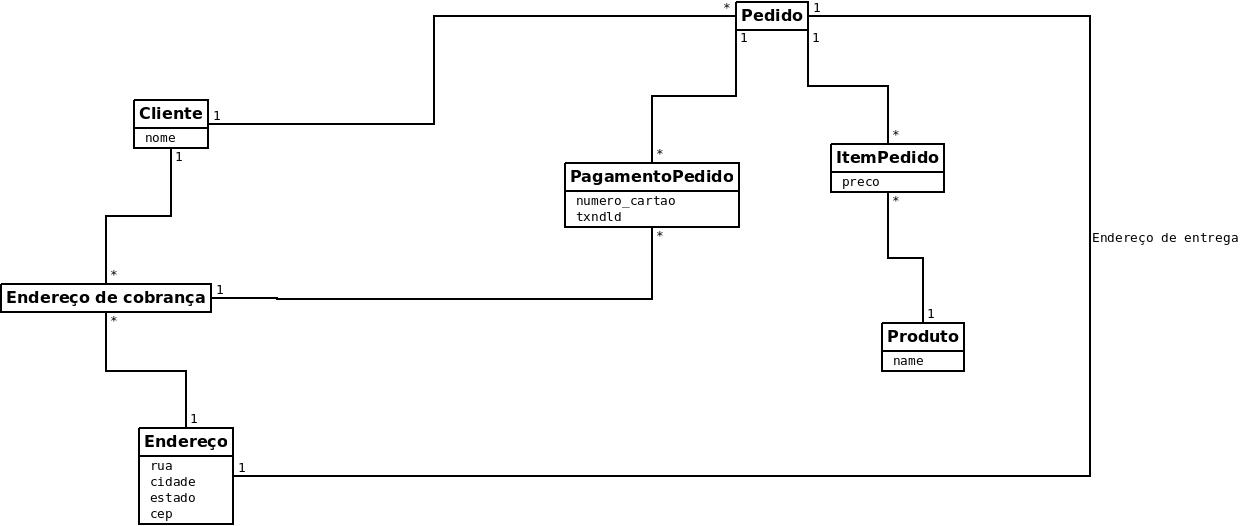
\includegraphics[width=\textwidth]{./04-figuras/diagrama_sql_uml.jpg}
    \fonte{\cite{NoSQL}}
    \label{fig:diagrama_sql_uml}
\end{figure}
\begin{figure}[!htb]
    \centering
    \caption{Exemplo da disposição dos dados no modelo relacional}
    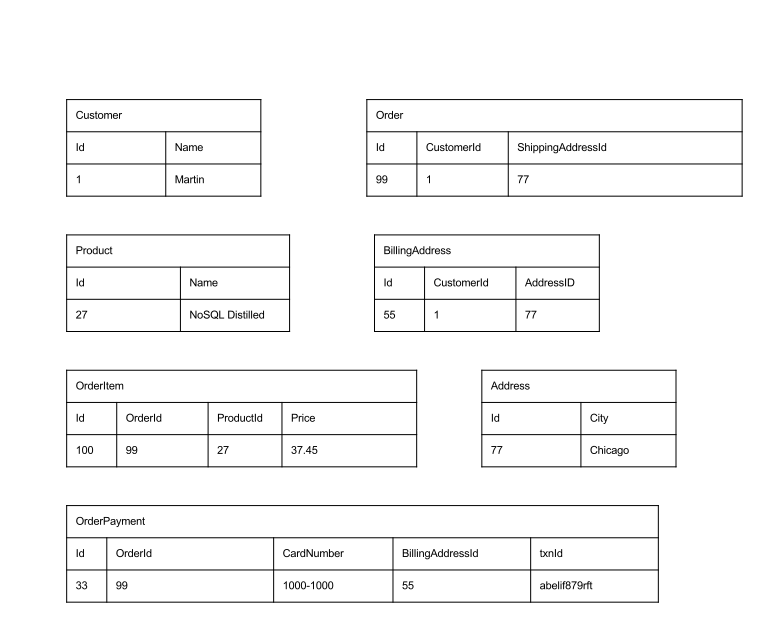
\includegraphics[width=\textwidth]{./04-figuras/disposicao_dados_tabela.png}
    \fonte{\cite{NoSQL}}
    \label{fig:disposicao_tabela}
\end{figure}


O gênero relacional funciona muito bem para diversas aplicações, pois é bem flexível em relação às consultas, permite concorrência, transações e pode ser integrado com várias aplicações. Porém, há uma desvantagem que causa frustação em muitos desenvolvedores, chamada de Impedância de Correspondência ou \textit{Impedance Mismatch}. Isso ocorre, pois nem sempre o tipo do campo no banco de dados irá corresponder com o tipo esperado da linguagem utilizada, então é necessário criar uma forma de associação entre o tipo da variável da linguagem com o tipo do valor da tabela. Outra desvantagem é que esse gênero não aceita valores multivalorados, distanciando a aplicação ainda mais do modelo relacional.


\subsection{Banco de dados não relacional}
\label{subsec:nosqldatabasetype}
Os bancos de dados NoSQL, foram construídos para suprir a necessidade de se trabalhar com grande quantidade de dados e em \textit{clusters}. NoSQL abrange diversos gêneros de banco de dados, entre eles o orientado a documento, chave-valor, orientado a coluna e orientado a nó.

Todos esses gêneros não possuem catálogo, ou seja, não é definido previamente qual estrutura dos dados que serão armazenados. Isso deixa o sistema mais flexível e permite que a estrutura dos dados seja facilmente alterada. É possível adicionar um novo campo, sem ter que preocupar com qual valor colocar para a base legada, pois os objetos de uma mesma coleção podem ter diferentes campos. Da mesma maneira, para remover um campo, basta parar de armazená-lo, pois os registros antigos, que tinha esse campo, continuarão com eles, e os objetos novos não irão armazenar esse campo que já não faz parte da aplicação \cite{NoSQL}.

Com isso é possível trabalhar com dados não uniformes: são dados que para cada registro há um conjunto diferente de atributos. Para que o banco de dados relacional lide objeto dessa natureza, seria necessário uma tabela com os campos de todos os objetos e consequentemente, isso traria uma quantidade grande de campos vazios.

Basicamente os banco de dados NoSQL deslocam a definição do esquema para a aplicação que acessa o banco. Isso pode se tornar problemático quando há muitas aplicações acessando o mesmo banco, mas existem soluções para resolver isso, como encapsular toda a interação com o banco de dados, fazendo esse funcionar como um \textit{web service}.


Também podemos dizer que o resultado mais importante do crescimento do NoSQL é a presistência poliglota \cite{NoSQL}.


O banco de dados orientado a documento
Agregação é uma coleção de objetos relacionados, que desejamos que seja tratado como uma unidade \cite{NoSQL}. Usando a agregação é possível armazenar atributos multivalorados. Normalmente desejamos que as operações de atualização sobre as agregações sejam atômicas.
Utilizando o mesmo exemplo de \textit{e-commerce} a cima o modelo UML para um banco de dados que permite a agregação seria como a figura 1 e a disposição desses dados seria como a figura

Falar do mongo, basear na documentação para explicar como funciona as relacoes e citar alguns estudo de caso do site


Falar do redis, basear no NoSQL e SDSW, mostrar alguns estudos de casos que estao no site



\subsection{Persistência Poliglota}
\label{subsec:polyglotpersitence}
Utilizar o NoSQL como base e fazer a comparaçao com o artigo de paradigma de programação
